\documentclass[]{article}

\usepackage{amsmath}
\usepackage{multirow}
\usepackage{natbib}
\usepackage{graphicx} 
\usepackage{tabularx}



\begin{document}

\title{Testing the Atomic Cooling Threshold with Globular Cluster Formation Epochs at z~9.6 and z~1.4}

\author{Denario}
\date{Anthropic, Gemini \& OpenAI servers. Planet Earth.}

\maketitle
\begin{abstract}
The formation of the first globular clusters (GCs) is hypothesized to be regulated by the atomic cooling threshold, which predicts their assembly in dark matter halos with virial temperatures exceeding $10^4$ K. We test this framework across cosmic time by comparing two distinct GC populations: the 19 clusters of the GEMS system observed at $z=9.625$ and the 5 clusters of the Sparkler system at $z=1.4$. By calculating the formation redshift ($z_{form}$) for each cluster from its published age, we map their empirical formation epochs onto the theoretical GC formation rate predicted by the model. We find the Sparkler GCs, with $z_{form}$ between 2.2 and 3.5, align with the predicted peak of formation activity, while the GEMS GCs, with $z_{form}$ between 9.7 and 19.1, populate the high-redshift tail of the same distribution, a result consistent with an observational selection effect. Furthermore, the GEMS clusters are unexpectedly more metal-rich than their lower-redshift Sparkler counterparts, implying their formation occurred within a massive and rapidly enriching host environment at cosmic dawn. The alignment of these two disparate populations with different epochs of a single theoretical framework suggests the atomic cooling threshold acts as a primary regulator of GC formation.
\end{abstract}








\section{Introduction}
\label{sec:intro}
Globular clusters (GCs) are dense, ancient stellar systems that serve as unique fossils of the early Universe. Within the standard cosmological model, their formation is thought to be intimately linked to the most intense star-forming episodes during the assembly of the first galaxies. A fundamental, yet unresolved, question in galaxy formation is what physical mechanism set the characteristic mass and time scales for the birth of these objects. A leading theoretical framework posits that the formation of the most ancient GCs was regulated by the atomic cooling threshold. This model predicts that efficient star formation, and by extension the assembly of GCs, could only occur within dark matter halos massive enough for their gas to cool via atomic hydrogen transitions. This process becomes effective when the halo's virial temperature, $T_{vir}$, exceeds approximately $10^4$ K, thereby establishing a minimum mass for the host environments of the first GCs. This physical threshold, in turn, predicts a characteristic cosmic history for GC formation, providing a falsifiable prediction that has been historically difficult to test at the relevant epochs.

The advent of powerful new observatories has recently made it possible to discover and characterize candidate GCs at the high redshifts where the predictions of the atomic cooling model are most prominent. Two such discoveries offer an unprecedented opportunity to test this framework across a vast expanse of cosmic time: the GEMS system, a collection of 19 proto-GC candidates observed at a redshift of $z=9.625$, and the Sparkler system, a group of 5 GCs observed at $z=1.4$. These two populations, separated by over eight billion years of cosmic evolution, provide distinct snapshots of the GC population. The GEMS clusters probe the era of cosmic dawn, when the first GCs were forming, while the Sparkler clusters represent a more mature population observed closer to the peak of cosmic star formation. If the atomic cooling threshold is a universal regulator, then the inferred formation histories of these two disparate systems should be consistent with a single, underlying theoretical prediction.

In this paper, we test the universality of the atomic cooling threshold by mapping the empirical formation epochs of the GEMS and Sparkler GCs onto the cosmic GC formation rate predicted by the model. For each cluster, we use its published age and observed redshift to calculate its formation redshift, $z_{form}$. This procedure allows us to place both the high-redshift GEMS population and the lower-redshift Sparkler population onto a common theoretical timeline. We find that the formation epochs of the Sparkler clusters align remarkably well with the predicted peak of GC formation activity. In contrast, the GEMS clusters populate the high-redshift tail of the same distribution, a result consistent with an observational selection effect favoring the discovery of the earliest-forming objects at high redshift. Furthermore, our analysis of the cluster metallicities reveals that the GEMS clusters are unexpectedly metal-rich for their early formation, implying they were born within a massive and rapidly enriching host environment. The consistency of these two distinct populations with a single theoretical framework provides strong evidence that the atomic cooling threshold is a primary physical process governing the formation of globular clusters.

\section{Methods}
\label{sec:methods}
This study combines published observational data for two distinct populations of globular clusters (GCs) with a theoretical model of GC formation. Our methodology is designed to place both populations onto a common temporal framework to test the universality of the atomic cooling threshold as a primary regulator of their formation. All calculations are performed assuming a flat $\Lambda$CDM cosmology consistent with the Planck 2018 results: $H_0 = 67.4$ km s$^{-1}$ Mpc$^{-1}$, $\Omega_m = 0.315$, and $\Omega_\Lambda = 0.685$.

\subsection{Globular cluster samples}
We utilize data for two systems of high-redshift GCs. The first is the GEMS system, comprising 19 proto-GC candidates observed at a redshift of $z_{obs} = 9.625$. The second is the Sparkler system, which consists of 5 GCs observed at $z_{obs} = 1.4$. For each of the 24 clusters across both samples, we use the published stellar mass ($M_\star$), age, and metallicity ($[\mathrm{Z/H}]$) as the basis for our analysis. These properties were derived from detailed spectral energy distribution fitting in their respective discovery papers.

\subsection{Calculation of formation redshifts}
A central component of our analysis is the conversion of each cluster's measured age and observed redshift into a formation redshift, $z_{form}$. This places all clusters, regardless of their observation epoch, onto a common timeline of cosmic history. The formation redshift is defined as the redshift at which the age of the Universe was equal to the lookback time to the cluster's formation. We calculate $z_{form}$ by numerically solving the following equation for each cluster:
\begin{equation}
    t_L(z_{form}) = t_L(z_{obs}) + \tau
\end{equation}
where $\tau$ is the published age of the cluster and $t_L(z)$ is the lookback time to a given redshift $z$, calculated as:
\begin{equation}
    t_L(z) = \frac{1}{H_0} \int_0^z \frac{dz'}{(1+z')\sqrt{\Omega_m(1+z')^3 + \Omega_\Lambda}}
\end{equation}
The asymmetric uncertainties on the published ages were propagated through this calculation to determine the corresponding asymmetric uncertainties on $z_{form}$.

\subsection{Theoretical model of gc formation}
To provide a theoretical context for our empirical results, we compare the distribution of formation redshifts to the cosmic GC formation rate predicted by the atomic cooling threshold model. This model posits that the formation of the first GCs is restricted to dark matter halos with a virial temperature $T_{vir} \geq 10^4$ K, the threshold at which gas can cool efficiently via atomic hydrogen line emission. We computed the theoretical GC formation rate as a function of redshift by calculating the abundance of these halos using the Sheth-Tormen halo mass function, implemented with the same Planck 2018 cosmological parameters used throughout our analysis. The resulting curve represents the predicted rate at which GCs form within halos massive enough to support atomic cooling across cosmic time.

\subsection{Statistical analysis}
We characterized the properties of the GEMS and Sparkler populations by calculating descriptive statistics (mean, median, and standard deviation) for their stellar masses, ages, metallicities, and derived formation redshifts. To investigate the relationship between stellar mass and chemical enrichment, we analyzed the mass-metallicity relation (MZR) for each system individually and for the combined sample. We performed a robust linear regression on the $[\mathrm{Z/H}]$ versus $\log_{10}(M_\star/M_\odot)$ data using the Theil-Sen estimator. This non-parametric method is insensitive to outliers and provides a reliable measure of the underlying trend in the data. The statistical significance of the resulting MZR slope was assessed using its 95\% confidence interval.

\section{Results}
\label{sec:results}
We present the results of our analysis, beginning with the derived formation redshifts for the GEMS and Sparkler globular cluster (GC) populations and their comparison to the theoretical atomic cooling model. We then summarize the statistical properties of the two samples and conclude with an analysis of their mass-metallicity relation.

\subsection{Formation epochs and the atomic cooling threshold}

For each of the 24 GCs in our combined sample, we calculated a formation redshift ($z_\mathrm{form}$) by converting its published age and observed redshift into a lookback time, assuming a Planck 2018 flat $\Lambda$CDM cosmology. The resulting properties for all clusters are listed in Table \ref{tab:gc_properties}. The GEMS clusters, observed at $z=9.625$, exhibit a wide range of formation redshifts, from $z_\mathrm{form} = 9.68$ to $19.13$, with a mean of $\langle z_\mathrm{form} \rangle = 12.90 \pm 2.44$. In contrast, the Sparkler clusters, observed at $z=1.4$, formed in a much narrower and later epoch, with $z_\mathrm{form}$ ranging from $2.18$ to $3.51$ and a mean of $\langle z_\mathrm{form} \rangle = 2.59 \pm 0.54$.

\begin{table*}[t]
\centering
\caption{Derived Properties of the GEMS and Sparkler Globular Clusters.}
\label{tab:gc_properties}
\resizebox{\textwidth}{!}{
\begin{tabular}{lccccccc}
\hline
\hline
GC ID & System & $\log_{10}(M_\star/M_\odot)$ & Age (Gyr) & $z_\mathrm{form}$ & $\sigma_{z,\mathrm{lo}}$ & $\sigma_{z,\mathrm{hi}}$ & $[\mathrm{Z/H}]$ \\
\hline
J1 & GEMS & 7.680 & 0.307 & 19.13 & $-2.07$ & $+3.89$ & $-0.156$ \\
I1 & GEMS & 7.210 & 0.222 & 14.55 & $-1.89$ & $+2.01$ & $-0.117$ \\
H1 & GEMS & 7.113 & 0.269 & 17.00 & $-2.55$ & $+2.73$ & $-0.167$ \\
G1 & GEMS & 6.580 & 0.091 & 10.55 & $-1.14$ & $+0.87$ & $-0.179$ \\
A1 & GEMS & 7.489 & 0.108 & 11.22 & $-0.55$ & $+0.52$ & $-0.205$ \\
B1 & GEMS & 8.048 & 0.208 & 13.73 & $-0.93$ & $+1.01$ & $-0.005$ \\
C1 & GEMS & 7.517 & 0.112 & 11.35 & $-0.77$ & $+0.80$ & $-0.060$ \\
D1 & GEMS & 7.883 & 0.220 & 14.38 & $-1.30$ & $+1.55$ & $-0.127$ \\
E1 & GEMS & 6.767 & 0.056 & 10.07 & $-0.82$ & $+0.49$ & $-0.185$ \\
F1 & GEMS & 6.909 & 0.098 & 10.87 & $-0.93$ & $+0.73$ & $-0.160$ \\
F2 & GEMS & 7.092 & 0.133 & 11.87 & $-0.66$ & $+0.79$ & $-0.271$ \\
E2 & GEMS & 6.202 & 0.004 & 9.68 & $-0.03$ & $+0.02$ & $-0.180$ \\
D2 & GEMS & 7.328 & 0.113 & 11.40 & $-1.07$ & $+1.01$ & $-0.167$ \\
C2 & GEMS & 7.575 & 0.116 & 11.49 & $-1.06$ & $+0.94$ & $-0.109$ \\
B2 & GEMS & 7.915 & 0.150 & 12.35 & $-0.56$ & $+0.60$ & $+0.041$ \\
A2 & GEMS & 7.224 & 0.090 & 10.52 & $-0.61$ & $+0.43$ & $-0.609$ \\
H2 & GEMS & 6.644 & 0.092 & 10.57 & $-1.31$ & $+0.74$ & $-0.237$ \\
I2 & GEMS & 7.273 & 0.248 & 15.87 & $-2.60$ & $+2.72$ & $-0.116$ \\
J2 & GEMS & 7.155 & 0.192 & 13.27 & $-1.14$ & $+1.44$ & $-0.155$ \\
\hline
1 & Sparkler & 6.891 & 2.731 & 3.51 & $-1.07$ & $+0.53$ & $-0.850$ \\
2 & Sparkler & 7.026 & 2.028 & 2.61 & $-0.44$ & $+0.36$ & $-0.483$ \\
4 & Sparkler & 6.847 & 1.509 & 2.18 & $-0.34$ & $+0.22$ & $-0.404$ \\
8 & Sparkler & 7.065 & 1.744 & 2.36 & $-0.31$ & $+0.25$ & $-0.965$ \\
10 & Sparkler & 6.944 & 1.660 & 2.29 & $-0.29$ & $+0.31$ & $-0.185$ \\
\hline
\end{tabular}
}
\end{table*}

To place these formation epochs in a theoretical context, we compare them to the cosmic GC formation rate predicted by the atomic cooling threshold model. This model, based on the abundance of dark matter halos with virial temperatures $T_\mathrm{vir} \geq 10^4$ K, predicts a formation rate that peaks broadly around $z \sim 3-6$ and declines at higher redshifts. Figure \ref{fig:image0}, panels (a) and (b), show the cumulative distribution of this theoretical formation rate, against which we plot the formation redshifts of our two GC samples.

The Sparkler GCs, with $z_\mathrm{form}$ between 2.2 and 3.5, align remarkably well with the predicted peak of GC formation activity. This finding supports the model's core prediction that a significant fraction of GCs formed in atomic cooling halos during the epoch of peak cosmic star formation.

Conversely, the GEMS GCs, with $z_\mathrm{form}$ spanning $\sim 9.7-19.1$, populate the high-redshift tail of the same theoretical distribution. This is not in tension with the model, but is a direct consequence of an observational selection effect: since the GEMS system is observed at $z_\mathrm{obs} = 9.625$, only clusters that formed at $z > 9.625$ are detectable. For instance, the youngest GEMS cluster (E2) has a formation redshift of $z_\mathrm{form} = 9.68$, only slightly higher than the observation redshift. The GEMS sample therefore exclusively probes the earliest phase of GC formation, corresponding to the assembly of the first atomic cooling halos in the most overdense regions of the early Universe. The existence of these clusters is fully consistent with the non-zero formation rate predicted by the model at these early times. The fact that both the Sparkler and GEMS populations align with different epochs of a single theoretical framework provides strong evidence for the universality of the atomic cooling threshold in regulating GC formation.

\begin{figure*}[t]
    \centering
    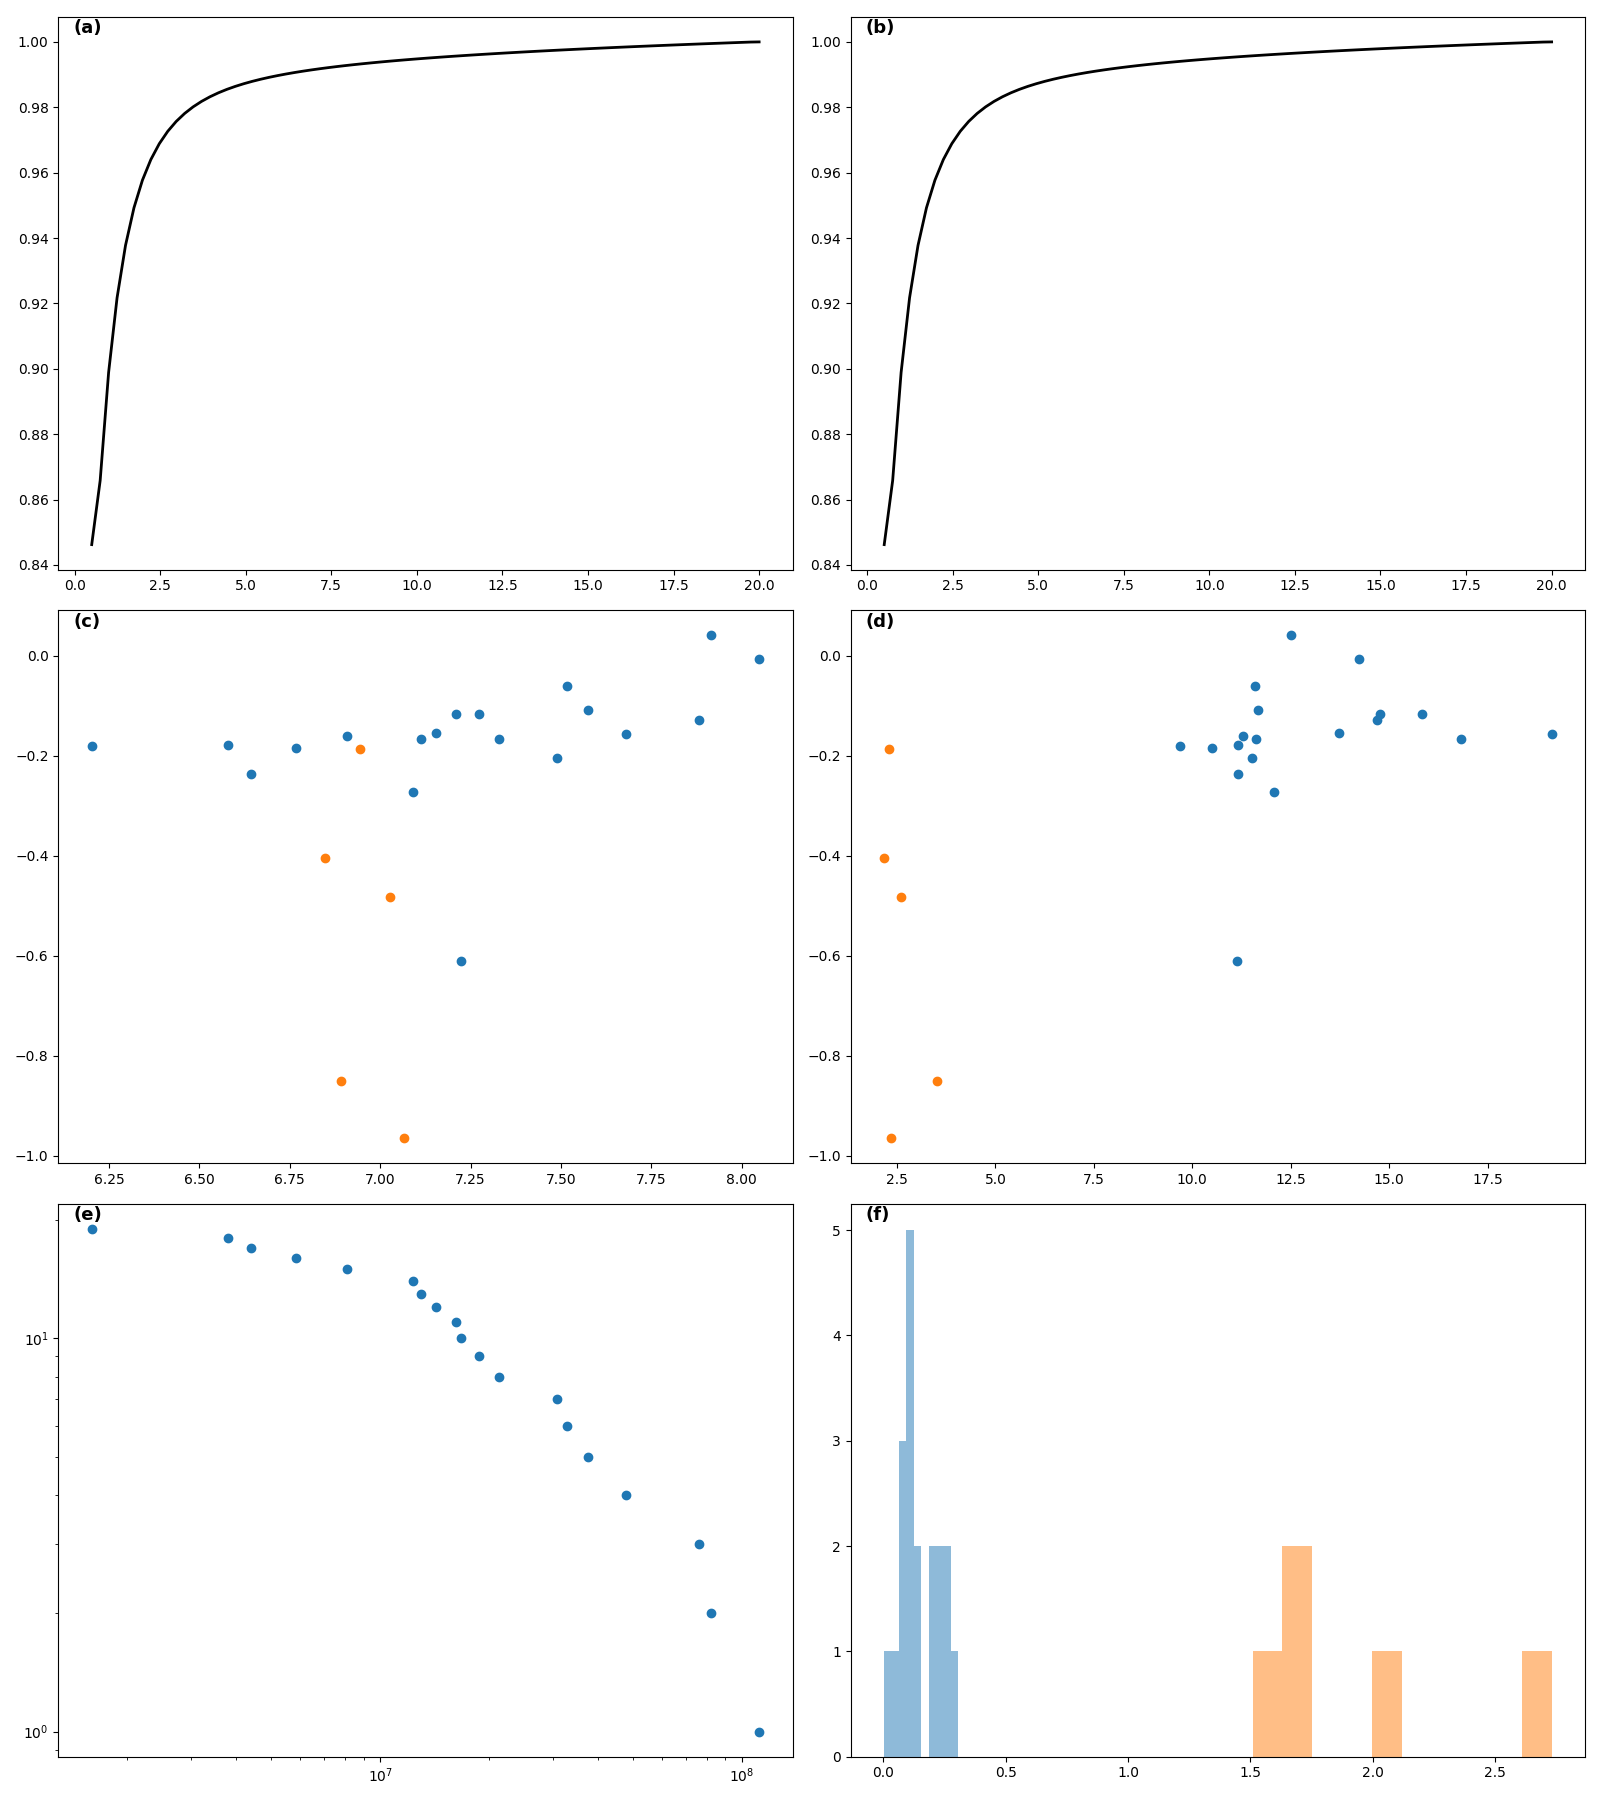
\includegraphics[width=\textwidth]{../input_files/plots/step_3_analysis_plot_1777372490.png}
    \caption{Properties of the GEMS (blue points) and Sparkler (orange points) globular cluster (GC) samples. Panels (a) and (b) show the cumulative formation history from the Trenti et al. (2015) atomic cooling model, with the formation redshifts of the GCs overplotted. Panel (c) displays the mass-metallicity relation, where GEMS GCs show a weak positive correlation. Panel (d) plots metallicity against formation redshift ($z_\mathrm{form}$), revealing that GEMS GCs formed earlier ($z_\mathrm{form} \approx 10-19$) yet are more metal-rich than the Sparkler GCs ($z_\mathrm{form} \approx 2-4$). Panel (e) shows the age-mass relation for the GEMS sample. Panel (f) presents the age distributions at the time of observation, demonstrating that GEMS GCs are very young (< 310 Myr) while Sparkler GCs are significantly older (> 1.5 Gyr).}
    \label{fig:image0}
\end{figure*}

\subsection{Physical properties of the GC populations}

A statistical summary of the key physical properties for both GC systems is provided in Table \ref{tab:summary_stats}. The two populations exhibit notable differences in their stellar mass, age, and metallicity distributions.

The GEMS system displays a wide diversity in stellar mass, spanning 1.85 dex from $\log_{10}(M_\star/M_\odot) = 6.20$ to $8.05$. In stark contrast, the Sparkler system is remarkably homogeneous in mass, with its five clusters spanning only 0.22 dex ($\log_{10}(M_\star/M_\odot) = 6.85$ to $7.07$).

The ages of the clusters at their respective observation redshifts also differ dramatically, as shown in Figure \ref{fig:image0}, panel (f). The GEMS GCs are exceptionally young, with ages ranging from just 4 Myr to 307 Myr. This indicates they are observed very soon after their formation. The Sparkler GCs, on the other hand, are much more evolved systems, with ages between 1.5 Gyr and 2.7 Gyr at $z=1.4$. Panel (e) of Figure \ref{fig:image0} shows the age-mass relation for the GEMS sample, revealing no significant correlation between the two properties.

Perhaps the most striking result is the difference in metallicity. As shown in Figure \ref{fig:image0}, panel (d), the GEMS clusters are systematically more metal-rich than their Sparkler counterparts, despite having formed at significantly higher redshifts. The GEMS sample has a median metallicity of $[\mathrm{Z/H}] = -0.160$, whereas the Sparkler sample has a median of $[\mathrm{Z/H}] = -0.483$. This counter-intuitive finding suggests that the GEMS clusters formed within a host environment that underwent extremely rapid and efficient chemical enrichment at cosmic dawn.

\begin{table*}[t]
\centering
\caption{Statistical Summary of GC Properties by System.}
\label{tab:summary_stats}
\begin{tabular}{lcccccc}
\hline
\hline
Property & GEMS (N=19) Mean & GEMS Median & GEMS Std. Dev. & Sparkler (N=5) Mean & Sparkler Median & Sparkler Std. Dev. \\
\hline
Age (Gyr) & 0.149 & 0.116 & 0.079 & 1.934 & 1.744 & 0.484 \\
$\log_{10}(M_\star/M_\odot)$ & 7.242 & 7.224 & 0.484 & 6.955 & 6.944 & 0.091 \\
$[\mathrm{Z/H}]$ & $-0.167$ & $-0.160$ & 0.130 & $-0.577$ & $-0.483$ & 0.323 \\
$z_\mathrm{form}$ & 12.90 & 11.67 & 2.44 & 2.59 & 2.36 & 0.54 \\
\hline
\end{tabular}
\end{table*}

\subsection{The mass-metallicity relation}

We investigated the relationship between stellar mass and metallicity for both systems, as shown in Figure \ref{fig:image0}, panel (c). Using a Theil-Sen robust linear regression, we find a weak but statistically significant positive correlation for the GEMS system. The slope is $+0.099$ dex per dex in stellar mass, with a 95\% confidence interval of $[+0.023, +0.184]$. This suggests that more massive GCs in the GEMS system are modestly more metal-rich, consistent with expectations from self-enrichment or formation within more massive, enriched sub-clumps.

For the Sparkler system, the regression is unconstrained due to the small sample size and narrow mass range. The resulting slope of $-1.616$ has an extremely wide 95\% confidence interval of $[-12.33, +12.56]$ and is consistent with a flat relation.

The overall mass-metallicity relation for the combined sample is driven by the GEMS clusters, yielding a positive slope of $+0.140$ (95\% CI: $[+0.033, +0.259]$). The most notable feature of the MZR plot is the clear offset between the two populations, with the GEMS clusters occupying a region of higher mass and significantly higher metallicity compared to the Sparkler clusters. This metallicity offset of $\sim 0.3-0.4$ dex at a fixed mass reinforces the conclusion that the GEMS clusters were born in a pre-enriched environment. The high metallicities ($[\mathrm{Z/H}] \sim -0.17$) at such early epochs ($z_\mathrm{form} \sim 10-19$) imply that their host halo was massive and experienced a rapid, intense burst of star formation and chemical enrichment in the first few hundred million years of cosmic history. This level of enrichment is remarkably high for this epoch; for comparison, the galaxy mass-metallicity relation of Maiolino et al. (2008) extrapolated to the median mass and formation redshift of the GEMS sample predicts a metallicity of only $[\mathrm{Z/H}] \approx -2.44$, highlighting the exceptionally enriched nature of the GEMS formation environment.

\section{Conclusions}
\label{sec:conclusions}


In this paper, we tested the hypothesis that the formation of globular clusters (GCs) is regulated by the atomic cooling threshold, which posits that GCs assemble in dark matter halos with virial temperatures exceeding $10^4$ K. To test this framework across cosmic time, we utilized published data for two distinct GC populations: the 19 proto-GC candidates of the GEMS system observed at $z=9.625$ and the 5 GCs of the Sparkler system at $z=1.4$. For each of the 24 clusters, we calculated its formation redshift, $z_{form}$, from its published age and observed redshift. We then compared the distribution of these empirical formation epochs to the theoretical cosmic GC formation rate predicted by the atomic cooling model.

Our analysis yields two primary findings. First, the formation epochs of the two GC populations are fully consistent with a single, continuous theoretical formation history predicted by the atomic cooling model. The Sparkler GCs, with formation redshifts between $z_{form} \approx 2.2$ and $3.5$, align with the predicted peak of GC formation activity. In contrast, the GEMS GCs, with formation redshifts spanning $z_{form} \approx 9.7$ to $19.1$, populate the high-redshift tail of the same distribution. This is consistent with an observational selection effect, as only clusters that formed prior to the observation epoch of $z=9.625$ can be detected in the GEMS sample. The existence of these early clusters is in agreement with the non-zero formation rate predicted by the model at cosmic dawn.

Second, we find a striking and counter-intuitive result regarding the chemical enrichment of these systems. The GEMS clusters, despite forming at significantly earlier cosmic times, are systematically more metal-rich (median $[\mathrm{Z/H}] = -0.160$) than their lower-redshift Sparkler counterparts (median $[\mathrm{Z/H}] = -0.483$). This implies that the GEMS clusters were born within a host environment that underwent extremely rapid and efficient chemical enrichment in the first few hundred million years of the Universe. Furthermore, we identify a weak but statistically significant positive mass-metallicity relation within the GEMS system, suggesting that its more massive clusters are modestly more enriched.

From these results, we conclude that the atomic cooling threshold appears to be a universal and primary physical mechanism governing the formation of GCs from cosmic dawn to the peak of cosmic star formation. The successful alignment of two disparate GC populations, separated by over eight billion years of cosmic evolution, with a single theoretical framework provides strong evidence for this model. The high metallicities of the GEMS clusters offer a powerful constraint on their formation environment, pointing to their assembly within a massive and rapidly evolving host halo at $z>9.6$. This study demonstrates the unique power of high-redshift GC populations to probe the fundamental physics of galaxy assembly in the early Universe.


\bibliography{bibliography}{}
\bibliographystyle{unsrt}

\end{document}
